\documentclass[12pt]{article}
\usepackage[margin=0.5in,landscape]{geometry}
\usepackage{tikz}
\usetikzlibrary{patterns,arrows.meta,decorations.pathreplacing,calc,positioning,
  patterns.meta}
\usepackage{amsmath,amssymb}
\usepackage{xcolor}
\usepackage{pgfplots}
\pgfplotsset{compat=1.18}

% Brand colors
\definecolor{garnet}{HTML}{73000A}
\definecolor{rose}{HTML}{CC2E40}
\definecolor{atlantic}{HTML}{466A9F}
\definecolor{congaree}{HTML}{1F414D}
\definecolor{horseshoe}{HTML}{65780B}
\definecolor{grass}{HTML}{CED318}
\definecolor{honeycomb}{HTML}{A49137}
\definecolor{gray90}{HTML}{363636}
\definecolor{gray70}{HTML}{5C5C5C}
\definecolor{gray50}{HTML}{A2A2A2}
\definecolor{gray30}{HTML}{C7C7C7}
\definecolor{gray10}{HTML}{ECECEC}
\definecolor{sandstorm}{HTML}{FFF2E3}

\pagestyle{empty}

\begin{document}

%% ============================================================
%% DIAGRAM 1 — CFAR Sliding Window (landscape, multi-position + variants)
%% ============================================================
\begin{center}
\textbf{\Large Diagram 1: CFAR Sliding Window}
\end{center}
\vspace{-0.1cm}

\begin{center}
\begin{tikzpicture}[scale=0.52, every node/.style={font=\small}]

% ====================================================================
% TOP SECTION: 1-D range line with power profile at THREE window positions
% ====================================================================
% Power values for 25-cell range line (indices 0..24)
% Two targets at cells 9 and 18, noise floor ~2-4
\def\pwr{{3,2,4,2,3,2,3,2,5,18,6,3,2,4,3,2,3,4,14,5,3,2,3,2,3}}
\def\Ncells{24}

% --- Power profile bar chart ---
\begin{scope}[shift={(0,19)}]
  \draw[-{Stealth[length=4pt]},gray70] (-0.3,0) -- (\Ncells*0.72+1,0);
  \draw[-{Stealth[length=4pt]},gray70] (-0.3,0) -- (-0.3,4.8);
  \node[font=\tiny,gray70] at (\Ncells*0.72+1.3,0) {Range bin};
  \node[font=\tiny,gray70,rotate=90] at (-0.7,2.4) {Power};

  % Noise floor shading
  \fill[gray10] (0,0) rectangle (\Ncells*0.72+0.65,0.7);
  \draw[gray30,dashed] (0,0.7) -- (\Ncells*0.72+0.65,0.7);
  \node[font=\tiny,gray50,right] at (\Ncells*0.72+0.7,0.7) {Noise floor};

  \foreach \i in {0,...,\Ncells}{
    \pgfmathtruncatemacro{\v}{\pwr[\i]}
    \pgfmathsetmacro{\h}{\v*0.24}
    \fill[gray30] (\i*0.72, 0) rectangle ++(0.62, \h);
    \draw[gray50,thin] (\i*0.72, 0) rectangle ++(0.62, \h);
    \node[font=\tiny,gray70] at (\i*0.72+0.31,-0.3) {\i};
  }

  % Target peaks labeled
  \fill[garnet] (9*0.72+0.31, 18*0.24+0.15) circle (0.15);
  \fill[garnet] (18*0.72+0.31, 14*0.24+0.15) circle (0.15);
\end{scope}

% --- Three window positions shown on cell strip ---
% Position 1: CUT=5 (no target), Position 2: CUT=9 (target), Position 3: CUT=18 (target)
\newcommand{\windowStrip}[3]{% #1=y-shift, #2=CUT index, #3=label
\begin{scope}[shift={(0,#1)}]
  \node[font=\footnotesize\bfseries,gray90,left] at (-0.5,0.4) {#3};
  \foreach \i in {0,...,\Ncells}{
    \pgfmathtruncatemacro{\v}{\pwr[\i]}
    % Zones: guard=CUT±1, leading=CUT-5..CUT-2, trailing=CUT+2..CUT+5
    \pgfmathtruncatemacro{\cutidx}{#2}
    \pgfmathtruncatemacro{\d}{\i-\cutidx}
    \pgfmathtruncatemacro{\absd}{abs(\d)}
    \pgfmathtruncatemacro{\iscut}{(\i==\cutidx)?1:0}
    \pgfmathtruncatemacro{\isguard}{(\absd>=1 && \absd<=1 && \iscut==0)?1:0}
    \pgfmathtruncatemacro{\islead}{(\d>=-5 && \d<=-2)?1:0}
    \pgfmathtruncatemacro{\istrail}{(\d>=2 && \d<=5)?1:0}
    %
    \ifnum\iscut=1
      \fill[garnet] (\i*0.72,0) rectangle ++(0.62,0.8);
    \else\ifnum\isguard=1
      \fill[gray50] (\i*0.72,0) rectangle ++(0.62,0.8);
    \else\ifnum\islead=1
      \fill[atlantic!50] (\i*0.72,0) rectangle ++(0.62,0.8);
    \else\ifnum\istrail=1
      \fill[congaree!40] (\i*0.72,0) rectangle ++(0.62,0.8);
    \else
      \fill[gray10] (\i*0.72,0) rectangle ++(0.62,0.8);
    \fi\fi\fi\fi
    \draw[gray70,thin] (\i*0.72,0) rectangle ++(0.62,0.8);
    \node[font=\tiny] at (\i*0.72+0.31,0.4) {\v};
  }
  % Braces
  \pgfmathtruncatemacro{\lstart}{#2-5}
  \pgfmathtruncatemacro{\lend}{#2-2}
  \pgfmathtruncatemacro{\tstart}{#2+2}
  \pgfmathtruncatemacro{\tend}{#2+5}
  \ifnum\lstart<0 \else
    \draw[decorate,decoration={brace,amplitude=3pt,mirror},atlantic,thick]
      (\lstart*0.72,-0.15) -- (\lend*0.72+0.62,-0.15);
    \node[below=3pt,font=\tiny,atlantic] at ({(\lstart+\lend)*0.36+0.31},-0.15) {Leading};
  \fi
  \ifnum\tend>\Ncells \else
    \draw[decorate,decoration={brace,amplitude=3pt,mirror},congaree,thick]
      (\tstart*0.72,-0.15) -- (\tend*0.72+0.62,-0.15);
    \node[below=3pt,font=\tiny,congaree] at ({(\tstart+\tend)*0.36+0.31},-0.15) {Trailing};
  \fi
  % Threshold arrow from CUT
  \pgfmathtruncatemacro{\cutval}{\pwr[\cutidx]}
  % Decision indicator
  \pgfmathtruncatemacro{\detected}{(\cutval>7)?1:0}
  \ifnum\detected=1
    \node[font=\small,horseshoe] at (\cutidx*0.72+0.31,1.2) {\checkmark};
  \else
    \node[font=\small,rose] at (\cutidx*0.72+0.31,1.2) {$\times$};
  \fi
\end{scope}
}

\windowStrip{14.5}{5}{Pos.\ 1: CUT\,=\,5}
\windowStrip{12.0}{9}{Pos.\ 2: CUT\,=\,9}
\windowStrip{9.5}{18}{Pos.\ 3: CUT\,=\,18}

% Sliding arrows between positions
\draw[-{Stealth[length=4pt]},rose,thick] (5*0.72+0.31,14.3) -- (9*0.72+0.31,12.95);
\draw[-{Stealth[length=4pt]},rose,thick] (9*0.72+0.31,11.8) -- (18*0.72+0.31,10.45);

% Legend for sliding window diagram
\begin{scope}[shift={(1,7.5)}]
  \fill[garnet] (0,0) rectangle ++(0.4,0.3);
  \node[right,font=\footnotesize] at (0.5,0.15) {CUT};
  %
  \fill[gray50] (2.2,0) rectangle ++(0.4,0.3);
  \node[right,font=\footnotesize] at (2.7,0.15) {Guard};
  %
  \fill[atlantic!50] (4.6,0) rectangle ++(0.4,0.3);
  \node[right,font=\footnotesize] at (5.1,0.15) {Leading};
  %
  \fill[congaree!40] (7.2,0) rectangle ++(0.4,0.3);
  \node[right,font=\footnotesize] at (7.7,0.15) {Trailing};
  %
  \node[font=\small,horseshoe] at (9.8,0.15) {\checkmark};
  \node[right,font=\footnotesize] at (10.0,0.15) {Detected};
  %
  \node[font=\small,rose] at (12,0.15) {$\times$};
  \node[right,font=\footnotesize] at (12.2,0.15) {Below $T$};
\end{scope}

\end{tikzpicture}
\end{center}

\newpage

%% ============================================================
%% DIAGRAM 1b — CFAR Variant Comparison (CA / GO / SO)
%% ============================================================
\begin{center}
\textbf{\Large Diagram 1b: CFAR Variant Comparison}
\end{center}
\vspace{-0.1cm}

\def\gsz{0.44}
\def\gn{10} % 0..10, center=5

% --- Three distinct power arrays for CA / GO / SO scenarios ---
% CA scene: uniform low clutter, target at center
\def\pwrCA{{2,1,2,1,2,1,2,1,2,1,2,
             1,2,1,2,2,2,2,2,1,2,1,
             2,1,2,2,3,3,3,2,2,1,2,
             1,2,2,3,3,3,3,3,2,2,1,
             2,2,3,3,3,4,3,3,3,2,2,
             1,2,3,3,4,15,4,3,3,2,1,
             2,2,3,3,3,4,3,3,3,2,2,
             1,2,2,3,3,3,3,3,2,2,1,
             2,1,2,2,3,3,3,2,2,1,2,
             1,2,1,2,2,2,2,2,1,2,1,
             2,1,2,1,2,1,2,1,2,1,2}}
% GO scene: strong interferer on leading (top) side
\def\pwrGO{{8,9,10,9,8,7,8,9,10,9,8,
             9,10,11,10,9,8,9,10,11,10,9,
             8,9,12,11,9,8,9,11,12,9,8,
             7,8,9,10,8,7,8,10,9,8,7,
             3,3,3,3,4,4,4,3,3,3,3,
             2,2,2,3,4,15,4,3,2,2,2,
             2,1,2,2,3,3,3,2,2,1,2,
             1,2,1,2,2,2,2,2,1,2,1,
             2,1,1,1,2,2,2,1,1,1,2,
             1,1,2,1,1,1,1,1,2,1,1,
             1,2,1,1,2,1,2,1,1,2,1}}
% SO scene: strong interferer on trailing (bottom) side
\def\pwrSO{{1,2,1,1,2,1,2,1,1,2,1,
             1,1,2,1,1,1,1,1,2,1,1,
             2,1,1,1,2,2,2,1,1,1,2,
             1,2,1,2,2,2,2,2,1,2,1,
             2,1,2,2,3,3,3,2,2,1,2,
             2,2,2,3,4,15,4,3,2,2,2,
             3,3,3,3,4,4,4,3,3,3,3,
             7,8,9,10,8,7,8,10,9,8,7,
             8,9,12,11,9,8,9,11,12,9,8,
             9,10,11,10,9,8,9,10,11,10,9,
             8,9,10,9,8,7,8,9,10,9,8}}

% === Raw intensity grid — takes x-offset, title, and macro name ===
% #1=x-offset, #2=title, #3=data macro (e.g. \pwrCA)
\newcommand{\rawGrid}[3]{%
\begin{scope}[shift={(#1,0)}]
  \node[font=\bfseries] at (5*\gsz+\gsz/2,\gn*\gsz+\gsz+0.4) {#2};
  \foreach \r in {0,...,\gn}{
    \foreach \c in {0,...,\gn}{
      \pgfmathtruncatemacro{\idx}{\r*11+\c}
      \pgfmathtruncatemacro{\val}{#3[\idx]}
      \pgfmathtruncatemacro{\cheb}{max(abs(\r-5),abs(\c-5))}
      \pgfmathtruncatemacro{\iscut}{(\cheb==0)?1:0}
      \pgfmathsetmacro{\pct}{min(\val*5.5,100)}
      \ifnum\iscut=1
        \fill[garnet] (\c*\gsz,\r*\gsz) rectangle ++(\gsz,\gsz);
        \node[font=\tiny,white] at (\c*\gsz+\gsz/2,\r*\gsz+\gsz/2) {\val};
      \else
        \fill[atlantic!\pct!white] (\c*\gsz,\r*\gsz) rectangle ++(\gsz,\gsz);
        \pgfmathtruncatemacro{\bright}{(\val>10)?1:0}
        \ifnum\bright=1
          \node[font=\tiny,white] at (\c*\gsz+\gsz/2,\r*\gsz+\gsz/2) {\val};
        \else
          \node[font=\tiny,black] at (\c*\gsz+\gsz/2,\r*\gsz+\gsz/2) {\val};
        \fi
      \fi
      \draw[gray70,very thin] (\c*\gsz,\r*\gsz) rectangle ++(\gsz,\gsz);
    }
  }
  \draw[garnet,very thick] (5*\gsz,5*\gsz) rectangle ++(\gsz,\gsz);
\end{scope}
}

% === CFAR variant grid (zone coloring, no annotations) ===
\newcommand{\varGrid}[3]{% #1=x-offset, #2=title, #3=mode 0=CA 1=GO 2=SO
\begin{scope}[shift={(#1,0)}]
  \node[font=\bfseries] at (5*\gsz+\gsz/2,\gn*\gsz+\gsz+0.4) {#2};

  \foreach \r in {0,...,\gn}{
    \foreach \c in {0,...,\gn}{
      \pgfmathtruncatemacro{\cheb}{max(abs(\r-5),abs(\c-5))}
      \pgfmathtruncatemacro{\iscut}{(\cheb==0)?1:0}
      \pgfmathtruncatemacro{\isguard}{(\cheb==1)?1:0}
      \pgfmathtruncatemacro{\isref}{(\cheb>=2 && \cheb<=4)?1:0}
      \pgfmathtruncatemacro{\islead}{(\r<5 && \isref==1)?1:0}
      \pgfmathtruncatemacro{\istrail}{(\r>5 && \isref==1)?1:0}
      \pgfmathtruncatemacro{\isside}{(\r==5 && \isref==1)?1:0}
      %
      \ifnum\iscut=1
        \fill[garnet] (\c*\gsz,\r*\gsz) rectangle ++(\gsz,\gsz);
      \else\ifnum\isguard=1
        \fill[gray50] (\c*\gsz,\r*\gsz) rectangle ++(\gsz,\gsz);
      \else
        % === CA ===
        \ifnum#3=0
          \ifnum\isref=1
            \fill[atlantic!45] (\c*\gsz,\r*\gsz) rectangle ++(\gsz,\gsz);
          \else
            \fill[gray10] (\c*\gsz,\r*\gsz) rectangle ++(\gsz,\gsz);
          \fi
        \fi
        % === GO: leading bold, trailing cross-hatched ===
        \ifnum#3=1
          \ifnum\islead=1
            \fill[atlantic!65] (\c*\gsz,\r*\gsz) rectangle ++(\gsz,\gsz);
          \else\ifnum\istrail=1
            \fill[atlantic!12] (\c*\gsz,\r*\gsz) rectangle ++(\gsz,\gsz);
            \fill[pattern=north east lines, pattern color=atlantic!30]
              (\c*\gsz,\r*\gsz) rectangle ++(\gsz,\gsz);
          \else\ifnum\isside=1
            \fill[atlantic!40] (\c*\gsz,\r*\gsz) rectangle ++(\gsz,\gsz);
          \else
            \fill[gray10] (\c*\gsz,\r*\gsz) rectangle ++(\gsz,\gsz);
          \fi\fi\fi
        \fi
        % === SO: trailing bold, leading cross-hatched ===
        \ifnum#3=2
          \ifnum\istrail=1
            \fill[atlantic!65] (\c*\gsz,\r*\gsz) rectangle ++(\gsz,\gsz);
          \else\ifnum\islead=1
            \fill[atlantic!12] (\c*\gsz,\r*\gsz) rectangle ++(\gsz,\gsz);
            \fill[pattern=north east lines, pattern color=atlantic!30]
              (\c*\gsz,\r*\gsz) rectangle ++(\gsz,\gsz);
          \else\ifnum\isside=1
            \fill[atlantic!40] (\c*\gsz,\r*\gsz) rectangle ++(\gsz,\gsz);
          \else
            \fill[gray10] (\c*\gsz,\r*\gsz) rectangle ++(\gsz,\gsz);
          \fi\fi\fi
        \fi
      \fi\fi
      \draw[gray70,very thin] (\c*\gsz,\r*\gsz) rectangle ++(\gsz,\gsz);
    }
  }

  % Zone boundary outlines
  \draw[garnet,very thick] (5*\gsz,5*\gsz) rectangle ++(\gsz,\gsz);
  \draw[gray90,thick,dashed] (4*\gsz,4*\gsz) rectangle ++(3*\gsz,3*\gsz);
  \draw[atlantic,thick] (1*\gsz,1*\gsz) rectangle ++(9*\gsz,9*\gsz);

  % Operator formula only
  \ifnum#3=0
    \node[font=\tiny] at (5.5*\gsz,-0.7)
      {$Z = \dfrac{1}{2N}\displaystyle\sum_{i=1}^{2N} x_i$};
  \fi
  \ifnum#3=1
    \node[font=\tiny] at (5.5*\gsz,-0.7)
      {$Z = \max\!\bigl(\bar{x}_L,\;\bar{x}_T\bigr)$};
  \fi
  \ifnum#3=2
    \node[font=\tiny] at (5.5*\gsz,-0.7)
      {$Z = \min\!\bigl(\bar{x}_L,\;\bar{x}_T\bigr)$};
  \fi
\end{scope}
}

\newsavebox{\cfarvariants}
\savebox{\cfarvariants}{%
\begin{tikzpicture}[every node/.style={font=\small,text=black}]

% --- TOP ROW: Raw intensity grids ---
\begin{scope}[shift={(0,7.5)}]
  \rawGrid{1}{Uniform Clutter}{\pwrCA}
  \rawGrid{7.5}{Strong Leading Edge}{\pwrGO}
  \rawGrid{14}{Strong Trailing Edge}{\pwrSO}
\end{scope}

% --- Downward arrows ---
\draw[-{Stealth[length=5pt]},gray70,thick]
  (1+5.5*\gsz, 7.2) -- (1+5.5*\gsz, 6.2);
\draw[-{Stealth[length=5pt]},gray70,thick]
  (7.5+5.5*\gsz, 7.2) -- (7.5+5.5*\gsz, 6.2);
\draw[-{Stealth[length=5pt]},gray70,thick]
  (14+5.5*\gsz, 7.2) -- (14+5.5*\gsz, 6.2);

% --- BOTTOM ROW: CFAR variant grids ---
\varGrid{1}{CA-CFAR}{0}
\varGrid{7.5}{GO-CFAR}{1}
\varGrid{14}{SO-CFAR}{2}

% Legend
\begin{scope}[shift={(1,-1.5)}]
  \fill[garnet] (0,0) rectangle ++(0.4,0.3);
  \node[right,font=\footnotesize] at (0.5,0.15) {CUT};
  %
  \fill[gray50] (2.2,0) rectangle ++(0.4,0.3);
  \node[right,font=\footnotesize] at (2.7,0.15) {Guard};
  %
  \fill[atlantic!65] (4.6,0) rectangle ++(0.4,0.3);
  \node[right,font=\footnotesize] at (5.1,0.15) {Selected Ref.};
  %
  \fill[atlantic!12] (7.8,0) rectangle ++(0.4,0.3);
  \fill[pattern=north east lines, pattern color=atlantic!30] (7.8,0) rectangle ++(0.4,0.3);
  \node[right,font=\footnotesize] at (8.3,0.15) {Unused Ref.};
\end{scope}

\end{tikzpicture}%
}% end savebox

\begin{center}
\resizebox{0.9\textwidth}{!}{\usebox{\cfarvariants}}
\end{center}

\newpage

%% ============================================================
%% DIAGRAM 2: Range-Azimuth to PPI Mapping (unchanged)
%% ============================================================
\begin{center}
\textbf{\Large Diagram 2: Range-Azimuth to PPI Mapping}
\end{center}
\vspace{0.2cm}

\begin{center}
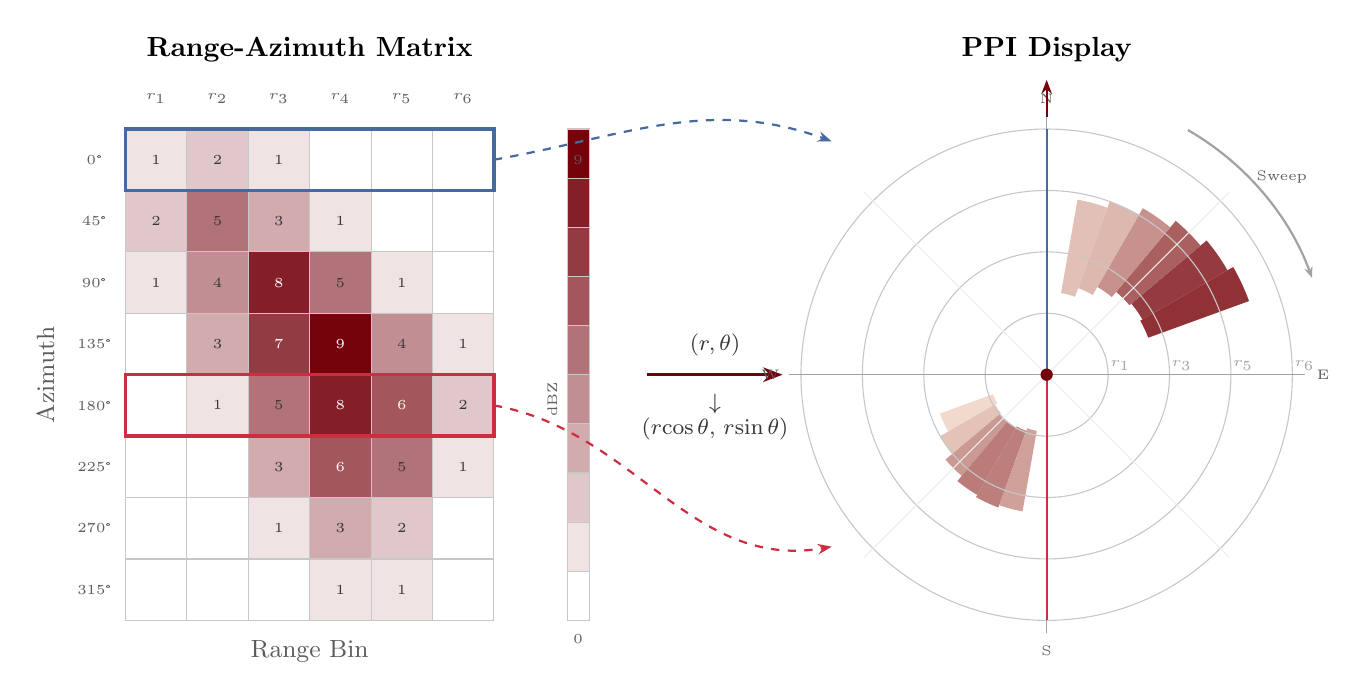
\begin{tikzpicture}[scale=0.78]

\node[font=\bfseries] at (3,9.3) {Range-Azimuth Matrix};

\def\rvals{{1,2,1,0,0,0,
             2,5,3,1,0,0,
             1,4,8,5,1,0,
             0,3,7,9,4,1,
             0,1,5,8,6,2,
             0,0,3,6,5,1,
             0,0,1,3,2,0,
             0,0,0,1,1,0}}

\foreach \r/\lbl in {7/$0$,6/$45$,5/$90$,4/$135$,3/$180$,2/$225$,1/$270$,0/$315$}{
  \node[font=\tiny,text=gray70] at (-0.5,\r+0.5) {\lbl\textdegree};
}
\foreach \c in {0,...,5}{
  \pgfmathtruncatemacro{\rb}{\c+1}
  \node[font=\tiny,text=gray70] at (\c+0.5,8.5) {$r_{\rb}$};
}

\foreach \r in {0,...,7}{
  \foreach \c in {0,...,5}{
    \pgfmathtruncatemacro{\idx}{\r*6+\c}
    \pgfmathtruncatemacro{\val}{\rvals[\idx]}
    \pgfmathsetmacro{\pct}{\val*11}
    \fill[garnet!\pct!white] (\c,7-\r) rectangle ++(1,1);
    \draw[gray30,thin] (\c,7-\r) rectangle ++(1,1);
    \ifnum\val>0
      \pgfmathtruncatemacro{\bright}{(\val>5)?1:0}
      \ifnum\bright=1
        \node[font=\tiny,white] at (\c+0.5,7.5-\r) {\val};
      \else
        \node[font=\tiny,gray90] at (\c+0.5,7.5-\r) {\val};
      \fi
    \fi
  }
}

\draw[atlantic,very thick] (0,7) rectangle ++(6,1);
\draw[rose,very thick] (0,3) rectangle ++(6,1);

\node[font=\small,text=gray70,rotate=90] at (-1.3,4) {Azimuth};
\node[font=\small,text=gray70] at (3,-0.5) {Range Bin};

\begin{scope}[shift={(7.2,0)}]
  \foreach \i in {0,...,9}{
    \pgfmathsetmacro{\pct}{\i*11}
    \fill[garnet!\pct!white] (0,\i*0.8) rectangle ++(0.35,0.8);
    \draw[gray30,thin] (0,\i*0.8) rectangle ++(0.35,0.8);
  }
  \node[font=\tiny,text=gray70] at (0.17,-0.3) {0};
  \node[font=\tiny,text=gray70] at (0.17,7.5) {9};
  \node[font=\tiny,text=gray70,rotate=90] at (-0.25,3.6) {dBZ};
\end{scope}

\begin{scope}[shift={(8.5,3.5)}]
  \draw[-{Stealth[length=7pt]},very thick,garnet] (0,0.5) -- (2.2,0.5);
  \node[font=\footnotesize,above,text=gray90] at (1.1,0.65) {$(r,\theta)$};
  \node[font=\footnotesize,below,text=gray90] at (1.1,0.35) {$\downarrow$};
  \node[font=\footnotesize,below,text=gray90] at (1.1,-0.05) {$(r\!\cos\theta,\,r\!\sin\theta)$};
\end{scope}

\begin{scope}[shift={(15,4)}]
  \node[font=\bfseries] at (0,5.3) {PPI Display};
  \foreach \a in {20,30,...,70}{
    \pgfmathsetmacro{\rin}{1.5+0.3*sin(\a*3)}
    \pgfmathsetmacro{\rout}{3.2+0.4*cos(\a*2)}
    \pgfmathsetmacro{\pct}{50+30*sin(\a*4)}
    \fill[garnet!\pct!sandstorm] (\a:\rin) -- (\a:\rout)
      arc[start angle=\a,end angle=\a+10,radius=\rout]
      -- (\a+10:\rin) arc[start angle=\a+10,end angle=\a,radius=\rin] -- cycle;
  }
  \foreach \a in {200,210,...,250}{
    \pgfmathsetmacro{\rin}{0.8+0.2*sin(\a*2)}
    \pgfmathsetmacro{\rout}{2.0+0.3*cos(\a*3)}
    \pgfmathsetmacro{\pct}{30+20*sin(\a*5)}
    \fill[garnet!\pct!sandstorm] (\a:\rin) -- (\a:\rout)
      arc[start angle=\a,end angle=\a+10,radius=\rout]
      -- (\a+10:\rin) arc[start angle=\a+10,end angle=\a,radius=\rin] -- cycle;
  }
  \foreach \rad/\lbl in {1/$r_1$,2/$r_3$,3/$r_5$,4/$r_6$}{
    \draw[gray30,thin] (0,0) circle (\rad);
    \node[font=\tiny,text=gray50] at (\rad+0.2,0.15) {\lbl};
  }
  \foreach \ang/\lbl in {90/N,0/E,270/S,180/W}{
    \draw[gray50,thin] (0,0) -- (\ang:4.2);
    \node[font=\tiny,text=gray70] at (\ang:4.5) {\lbl};
  }
  \foreach \ang in {45,135,225,315}{
    \draw[gray10,thin] (0,0) -- (\ang:4.2);
  }
  \draw[atlantic,thick] (0,0) -- (90:4);
  \draw[rose,thick] (0,0) -- (270:4);
  \draw[-{Stealth[length=5pt]},thick,garnet] (0,4.2) -- (0,4.8);
  \fill[garnet] (0,0) circle (0.1);
  \draw[-{Stealth[length=4pt]},gray50,thick] (60:4.6) arc[start angle=60,end angle=20,radius=4.6];
  \node[font=\tiny,gray70] at (40:5.0) {Sweep};
\end{scope}

\draw[-{Stealth[length=5pt]},dashed,atlantic,thick]
  (6,7.5) to[out=10,in=160] (11.5,7.8);
\draw[-{Stealth[length=5pt]},dashed,rose,thick]
  (6,3.5) to[out=-10,in=190] (11.5,1.2);

\end{tikzpicture}
\end{center}

\newpage

%% ============================================================
%% DIAGRAM 3 — Coverage Scoring (landscape, richer)
%% ============================================================
\begin{center}
\textbf{\Large Diagram 3: Coverage Score Illustration}
\end{center}
\vspace{-0.1cm}

\begin{center}
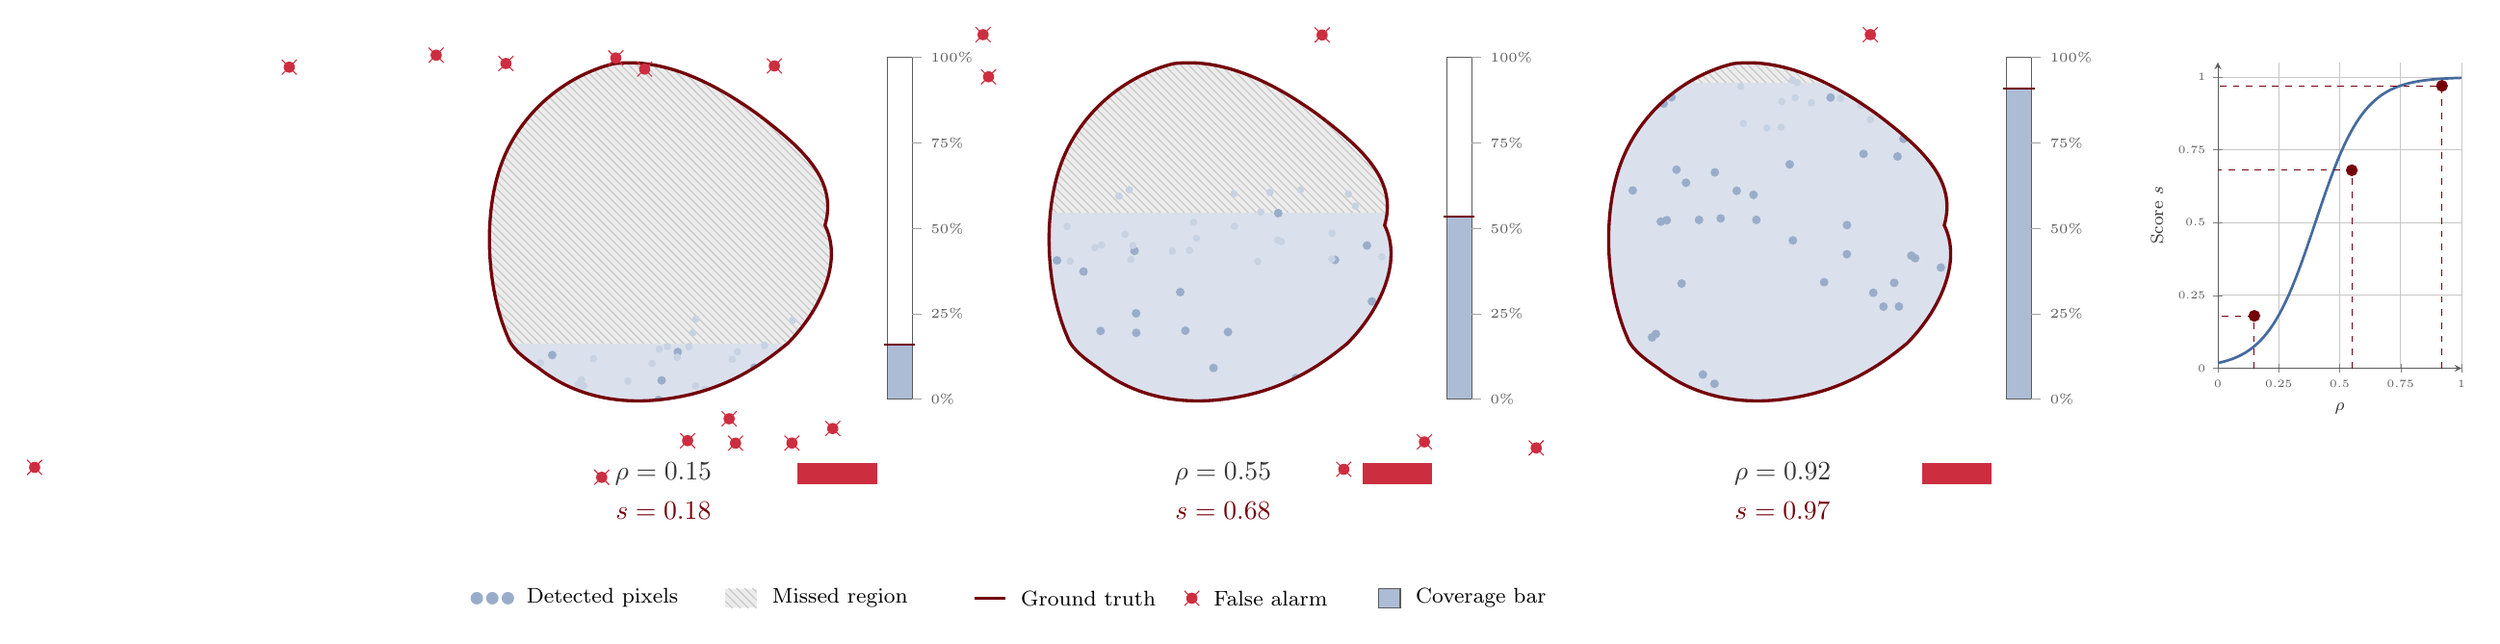
\begin{tikzpicture}[scale=0.82, every node/.style={font=\small}]

% --- Irregular weather-return blob (more complex shape) ---
\def\blobpath{
  (0.5,1.0) .. controls (0.15,1.8) and (0.1,3.0) ..
  (0.4,3.8) .. controls (0.7,4.6) and (1.4,5.2) ..
  (2.2,5.4) .. controls (3.0,5.5) and (3.8,5.1) ..
  (4.5,4.6) .. controls (5.3,4.0) and (5.8,3.5) ..
  (5.6,2.8) .. controls (5.9,2.2) and (5.5,1.4) ..
  (5.0,0.9) .. controls (4.4,0.4) and (3.8,0.1) ..
  (3.0,0.0) .. controls (2.2,-0.1) and (1.5,0.1) ..
  (1.0,0.5) .. controls (0.7,0.7) and (0.55,0.85) ..
  (0.5,1.0)
}

% ===============================================================
% PANEL MACRO
% ===============================================================
\newcommand{\covPanel}[6]{%
  % #1=xshift, #2=rho, #3=score, #4=fill-height, #5=seed, #6=num-false-alarms
  \begin{scope}[shift={(#1,0)}]

    % --- Unfilled interior (missed) ---
    \begin{scope}
      \clip \blobpath;
      \fill[gray10] (-0.5,-1) rectangle (7,6.5);
      % Missed-region crosshatch above fill line
      \fill[pattern=north west lines, pattern color=gray30]
        (-0.5,#4) rectangle (7,6.5);
    \end{scope}

    % --- Detected: scattered dots (not solid fill) ---
    \begin{scope}
      \clip \blobpath;
      % Base tint
      \fill[atlantic!20] (-0.5,-1) rectangle (7,#4);
      % Scattered detection pixels
      \pgfmathseed{#5}
      \foreach \i in {1,...,200}{
        \pgfmathsetmacro{\px}{-0.2+rand*6.2}
        \pgfmathsetmacro{\py}{-0.3+rand*5.8}
        \pgfmathsetmacro{\ht}{#4}
        \ifdim\py pt<\ht pt
          \fill[atlantic!55] (\px,\py) circle (0.07);
        \fi
      }
      % Sparser fringe dots near boundary
      \foreach \i in {1,...,50}{
        \pgfmathsetmacro{\px}{-0.1+rand*6.0}
        \pgfmathsetmacro{\py}{#4 - 0.2 + rand*0.6}
        \fill[atlantic!30] (\px,\py) circle (0.06);
      }
    \end{scope}

    % --- Ground truth outline ---
    \draw[garnet, very thick] \blobpath;

    % --- False alarms outside blob ---
    \pgfmathseed{#5}
    \foreach \i in {1,...,#6}{
      \pgfmathsetmacro{\fx}{-0.6+rand*7.0}
      \pgfmathsetmacro{\fy}{-0.8+rand*0.6}
      \fill[rose] (\fx,\fy) circle (0.09);
      \draw[rose,thin] (\fx-0.12,\fy-0.12) -- (\fx+0.12,\fy+0.12);
      \draw[rose,thin] (\fx-0.12,\fy+0.12) -- (\fx+0.12,\fy-0.12);
    }
    % Top-side false alarms
    \foreach \i in {1,...,#6}{
      \pgfmathsetmacro{\fx}{0.5+rand*4.5}
      \pgfmathsetmacro{\fy}{5.5+rand*0.5}
      \fill[rose] (\fx,\fy) circle (0.09);
      \draw[rose,thin] (\fx-0.12,\fy-0.12) -- (\fx+0.12,\fy+0.12);
      \draw[rose,thin] (\fx-0.12,\fy+0.12) -- (\fx+0.12,\fy-0.12);
    }

    % --- Coverage thermometer bar ---
    \begin{scope}[shift={(6.6,0)}]
      \draw[gray30] (0,0) rectangle (0.4,5.5);
      \pgfmathsetmacro{\barh}{#4*0.98}
      \fill[atlantic!45] (0,0) rectangle (0.4,\barh);
      \draw[gray70,thin] (0,0) rectangle (0.4,5.5);
      % Ticks
      \foreach \frac/\lbl in {0/0,1.375/25,2.75/50,4.125/75,5.5/100}{
        \draw[gray50] (0.4,\frac) -- (0.55,\frac);
        \node[right,font=\tiny,gray70] at (0.55,\frac) {\lbl\%};
      }
      % Marker line at current fill
      \draw[garnet,thick] (-0.05,\barh) -- (0.45,\barh);
    \end{scope}

    % --- FA count badge ---
    \pgfmathtruncatemacro{\facount}{#6*2}
    \node[draw=rose,fill=rose!10,font=\tiny\bfseries,rose,
      inner sep=2pt] at (5.8,-1.2) {FA\,=\,\facount};

    % --- Labels ---
    \node[font=\normalsize,text=gray90] at (3,-1.2) {$\rho = #2$};
    \node[font=\normalsize\bfseries,text=garnet] at (3,-1.8) {$s = #3$};
  \end{scope}
}

\covPanel{0}{0.15}{0.18}{0.9}{42}{6}
\covPanel{9}{0.55}{0.68}{3.0}{137}{3}
\covPanel{18}{0.92}{0.97}{5.1}{253}{1}

% --- Score curve (rho vs score) ---
\begin{scope}[shift={(28,0.5)}]
  \begin{axis}[
    width=5.5cm, height=6.5cm,
    xlabel={$\rho$},
    ylabel={Score $s$},
    xmin=0, xmax=1, ymin=0, ymax=1.05,
    xtick={0,0.25,0.5,0.75,1.0},
    ytick={0,0.25,0.5,0.75,1.0},
    grid=major,
    grid style={gray30,thin},
    axis lines=left,
    every axis label/.style={font=\footnotesize,text=gray90},
    tick label style={font=\tiny,text=gray70},
    axis line style={gray70},
  ]
    % Score curve (sigmoid-like)
    \addplot[domain=0:1, samples=80, very thick, atlantic]
      {1/(1+exp(-10*(x-0.4)))};
    % Operating points
    \addplot[only marks, mark=*, mark size=2.5pt, garnet]
      coordinates {(0.15,0.18) (0.55,0.68) (0.92,0.97)};
    % Dashed drop lines
    \draw[garnet,dashed,thin] (axis cs:0.15,0) -- (axis cs:0.15,0.18)
      -- (axis cs:0,0.18);
    \draw[garnet,dashed,thin] (axis cs:0.55,0) -- (axis cs:0.55,0.68)
      -- (axis cs:0,0.68);
    \draw[garnet,dashed,thin] (axis cs:0.92,0) -- (axis cs:0.92,0.97)
      -- (axis cs:0,0.97);
  \end{axis}
\end{scope}

% ---- LEGEND ----
\begin{scope}[shift={(0,-3.2)}]
  \fill[atlantic!55] (0,0) circle (0.1);
  \fill[atlantic!55] (0.25,0) circle (0.1);
  \fill[atlantic!55] (0.5,0) circle (0.1);
  \node[right,font=\footnotesize] at (0.65,0) {Detected pixels};
  %
  \fill[gray10] (4,-.15) rectangle ++(0.5,0.3);
  \fill[pattern=north west lines, pattern color=gray30] (4,-.15) rectangle ++(0.5,0.3);
  \node[right,font=\footnotesize] at (4.6,0) {Missed region};
  %
  \draw[garnet,very thick] (8,0) -- ++(0.5,0);
  \node[right,font=\footnotesize] at (8.6,0) {Ground truth};
  %
  \fill[rose] (11.5,0) circle (0.09);
  \draw[rose,thin] (11.5-0.12,-0.12) -- (11.5+0.12,0.12);
  \draw[rose,thin] (11.5-0.12,0.12) -- (11.5+0.12,-0.12);
  \node[right,font=\footnotesize] at (11.7,0) {False alarm};
  %
  \fill[atlantic!45] (14.5,-0.15) rectangle ++(0.35,0.3);
  \draw[gray70,thin] (14.5,-0.15) rectangle ++(0.35,0.3);
  \node[right,font=\footnotesize] at (14.95,0) {Coverage bar};
\end{scope}

\end{tikzpicture}
\end{center}

\newpage

%% ============================================================
%% DIAGRAM 4: Guard Cell Size Effect (unchanged)
%% ============================================================
\begin{center}
\textbf{\Large Diagram 4: Guard Cell Size Effect}
\end{center}
\vspace{0.2cm}

\begin{center}
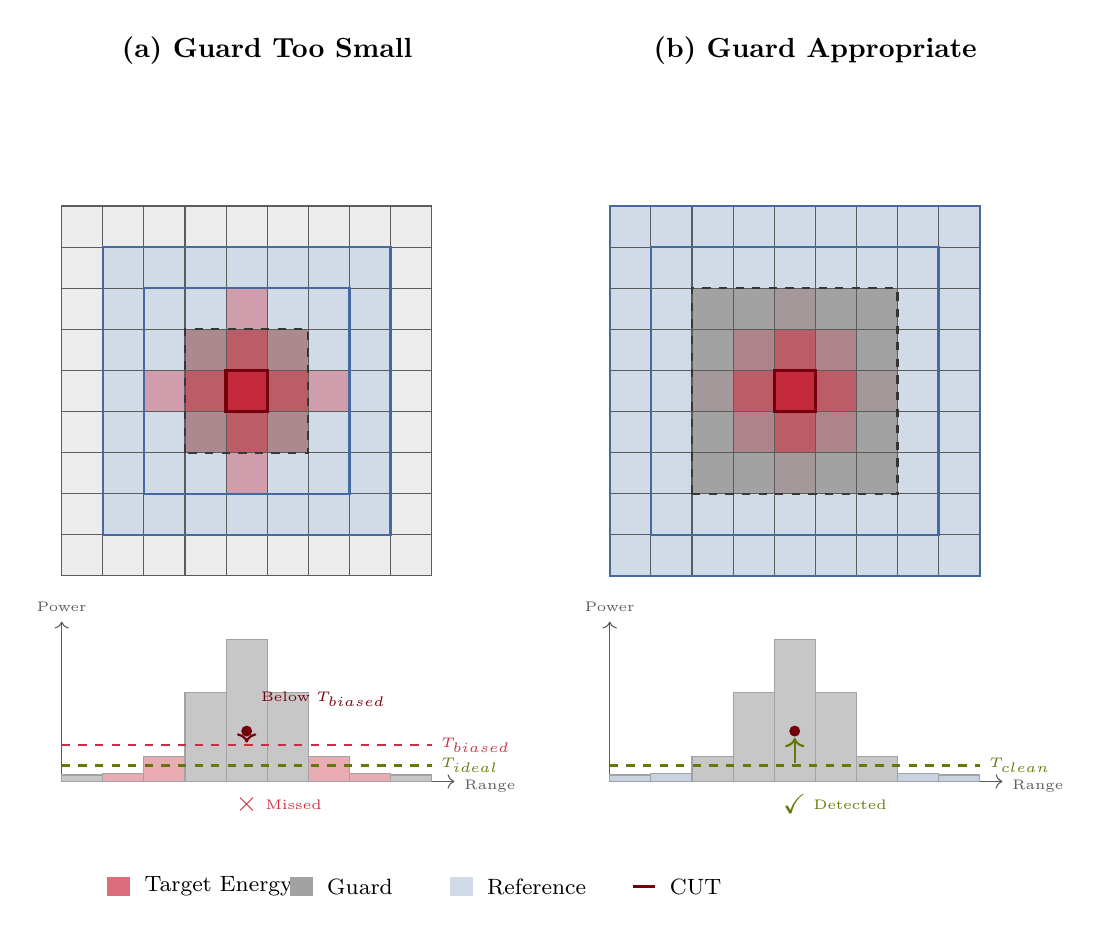
\begin{tikzpicture}[scale=0.58]

\begin{scope}[shift={(0,0)}]
  \node[font=\bfseries] at (4.5,11.5) {(a) Guard Too Small};
  \def\sz{0.9}
  \foreach \r in {0,...,8}{
    \foreach \c in {0,...,8}{
      \pgfmathtruncatemacro{\cheb}{max(abs(\r-4),abs(\c-4))}
      \pgfmathtruncatemacro{\iscut}{(\cheb==0)?1:0}
      \pgfmathtruncatemacro{\isguard}{(\cheb==1)?1:0}
      \pgfmathtruncatemacro{\isref}{(\cheb>=2 && \cheb<=3)?1:0}
      \ifnum\iscut=1
        \fill[garnet] (\c*\sz,\r*\sz) rectangle ++(\sz,\sz);
      \else\ifnum\isguard=1
        \fill[gray50] (\c*\sz,\r*\sz) rectangle ++(\sz,\sz);
      \else\ifnum\isref=1
        \fill[atlantic!25] (\c*\sz,\r*\sz) rectangle ++(\sz,\sz);
      \else
        \fill[gray10] (\c*\sz,\r*\sz) rectangle ++(\sz,\sz);
      \fi\fi\fi
      \draw[gray70,thin] (\c*\sz,\r*\sz) rectangle ++(\sz,\sz);
    }
  }
  \fill[rose,opacity=0.9] (4*\sz,4*\sz) rectangle ++(\sz,\sz);
  \fill[rose,opacity=0.6] (3*\sz,4*\sz) rectangle ++(\sz,\sz);
  \fill[rose,opacity=0.6] (5*\sz,4*\sz) rectangle ++(\sz,\sz);
  \fill[rose,opacity=0.6] (4*\sz,3*\sz) rectangle ++(\sz,\sz);
  \fill[rose,opacity=0.6] (4*\sz,5*\sz) rectangle ++(\sz,\sz);
  \fill[rose,opacity=0.35] (2*\sz,4*\sz) rectangle ++(\sz,\sz);
  \fill[rose,opacity=0.35] (6*\sz,4*\sz) rectangle ++(\sz,\sz);
  \fill[rose,opacity=0.35] (4*\sz,2*\sz) rectangle ++(\sz,\sz);
  \fill[rose,opacity=0.35] (4*\sz,6*\sz) rectangle ++(\sz,\sz);
  \fill[rose,opacity=0.2] (3*\sz,3*\sz) rectangle ++(\sz,\sz);
  \fill[rose,opacity=0.2] (5*\sz,5*\sz) rectangle ++(\sz,\sz);
  \fill[rose,opacity=0.2] (3*\sz,5*\sz) rectangle ++(\sz,\sz);
  \fill[rose,opacity=0.2] (5*\sz,3*\sz) rectangle ++(\sz,\sz);
  \foreach \r in {0,...,8}{
    \foreach \c in {0,...,8}{
      \draw[gray70,thin] (\c*\sz,\r*\sz) rectangle ++(\sz,\sz);
    }
  }
  \draw[garnet,very thick] (4*\sz,4*\sz) rectangle ++(\sz,\sz);
  \draw[gray90,thick,dashed] (3*\sz,3*\sz) rectangle ++(3*\sz,3*\sz);
  \draw[atlantic,thick] (2*\sz,2*\sz) rectangle ++(5*\sz,5*\sz);
  \draw[atlantic,thick] (1*\sz,1*\sz) rectangle ++(7*\sz,7*\sz);

  \begin{scope}[shift={(0,-4.5)}]
    \draw[->,gray70] (0,0) -- (9*\sz+0.5,0);
    \draw[->,gray70] (0,0) -- (0,3.5);
    \node[font=\tiny,gray70,right] at (9*\sz+0.5,-0.1) {Range};
    \node[font=\tiny,gray70,above] at (0,3.5) {Power};
    \foreach \i in {0,...,8}{
      \pgfmathsetmacro{\xp}{\i*\sz}
      \pgfmathsetmacro{\pw}{0.4+8.5*exp(-(\i-4)*(\i-4)/2.0)}
      \pgfmathtruncatemacro{\cheb}{abs(\i-4)}
      \pgfmathtruncatemacro{\isref}{(\cheb>=2 && \cheb<=3)?1:0}
      \ifnum\isref=1
        \fill[rose!40] (\xp,0) rectangle ++(\sz,\pw*0.35);
      \else
        \fill[gray30] (\xp,0) rectangle ++(\sz,\pw*0.35);
      \fi
      \draw[gray50,thin] (\xp,0) rectangle ++(\sz,\pw*0.35);
    }
    \draw[horseshoe,thick,dashed] (0,0.35) -- (9*\sz,0.35);
    \node[font=\tiny,horseshoe,right] at (9*\sz,0.35) {$T_{ideal}$};
    \draw[rose,thick,dashed] (0,0.8) -- (9*\sz,0.8);
    \node[font=\tiny,rose,right] at (9*\sz,0.8) {$T_{biased}$};
    \fill[garnet] (4*\sz+\sz/2, 3.15*0.35) circle (0.12);
    \draw[->,garnet,thick] (4*\sz+\sz/2, 3.15*0.35-0.15) -- (4*\sz+\sz/2, 0.85);
    \node[font=\tiny,garnet,right] at (4*\sz+\sz/2+0.1,1.8) {Below $T_{biased}$};
    \node[font=\normalsize,rose] at (4*\sz+\sz/2, -0.5) {$\times$};
    \node[font=\tiny,rose,right] at (4*\sz+\sz/2+0.2, -0.5) {Missed};
  \end{scope}
\end{scope}

\begin{scope}[shift={(12,0)}]
  \node[font=\bfseries] at (4.5,11.5) {(b) Guard Appropriate};
  \def\sz{0.9}
  \foreach \r in {0,...,8}{
    \foreach \c in {0,...,8}{
      \pgfmathtruncatemacro{\cheb}{max(abs(\r-4),abs(\c-4))}
      \pgfmathtruncatemacro{\iscut}{(\cheb==0)?1:0}
      \pgfmathtruncatemacro{\isguard}{(\cheb>=1 && \cheb<=2)?1:0}
      \pgfmathtruncatemacro{\isref}{(\cheb>=3 && \cheb<=4)?1:0}
      \ifnum\iscut=1
        \fill[garnet] (\c*\sz,\r*\sz) rectangle ++(\sz,\sz);
      \else\ifnum\isguard=1
        \fill[gray50] (\c*\sz,\r*\sz) rectangle ++(\sz,\sz);
      \else\ifnum\isref=1
        \fill[atlantic!25] (\c*\sz,\r*\sz) rectangle ++(\sz,\sz);
      \else
        \fill[gray10] (\c*\sz,\r*\sz) rectangle ++(\sz,\sz);
      \fi\fi\fi
      \draw[gray70,thin] (\c*\sz,\r*\sz) rectangle ++(\sz,\sz);
    }
  }
  \fill[rose,opacity=0.9] (4*\sz,4*\sz) rectangle ++(\sz,\sz);
  \fill[rose,opacity=0.6] (3*\sz,4*\sz) rectangle ++(\sz,\sz);
  \fill[rose,opacity=0.6] (5*\sz,4*\sz) rectangle ++(\sz,\sz);
  \fill[rose,opacity=0.6] (4*\sz,3*\sz) rectangle ++(\sz,\sz);
  \fill[rose,opacity=0.6] (4*\sz,5*\sz) rectangle ++(\sz,\sz);
  \fill[rose,opacity=0.25] (3*\sz,3*\sz) rectangle ++(\sz,\sz);
  \fill[rose,opacity=0.25] (5*\sz,5*\sz) rectangle ++(\sz,\sz);
  \fill[rose,opacity=0.25] (3*\sz,5*\sz) rectangle ++(\sz,\sz);
  \fill[rose,opacity=0.25] (5*\sz,3*\sz) rectangle ++(\sz,\sz);
  \fill[rose,opacity=0.08] (2*\sz,4*\sz) rectangle ++(\sz,\sz);
  \fill[rose,opacity=0.08] (6*\sz,4*\sz) rectangle ++(\sz,\sz);
  \fill[rose,opacity=0.08] (4*\sz,2*\sz) rectangle ++(\sz,\sz);
  \fill[rose,opacity=0.08] (4*\sz,6*\sz) rectangle ++(\sz,\sz);
  \foreach \r in {0,...,8}{
    \foreach \c in {0,...,8}{
      \draw[gray70,thin] (\c*\sz,\r*\sz) rectangle ++(\sz,\sz);
    }
  }
  \draw[garnet,very thick] (4*\sz,4*\sz) rectangle ++(\sz,\sz);
  \draw[gray90,thick,dashed] (2*\sz,2*\sz) rectangle ++(5*\sz,5*\sz);
  \draw[atlantic,thick] (1*\sz,1*\sz) rectangle ++(7*\sz,7*\sz);
  \draw[atlantic,thick] (0*\sz,0*\sz) rectangle ++(9*\sz,9*\sz);

  \begin{scope}[shift={(0,-4.5)}]
    \draw[->,gray70] (0,0) -- (9*\sz+0.5,0);
    \draw[->,gray70] (0,0) -- (0,3.5);
    \node[font=\tiny,gray70,right] at (9*\sz+0.5,-0.1) {Range};
    \node[font=\tiny,gray70,above] at (0,3.5) {Power};
    \foreach \i in {0,...,8}{
      \pgfmathsetmacro{\xp}{\i*\sz}
      \pgfmathsetmacro{\pw}{0.4+8.5*exp(-(\i-4)*(\i-4)/2.0)}
      \pgfmathtruncatemacro{\cheb}{abs(\i-4)}
      \pgfmathtruncatemacro{\isref}{(\cheb>=3 && \cheb<=4)?1:0}
      \ifnum\isref=1
        \fill[atlantic!30] (\xp,0) rectangle ++(\sz,\pw*0.35);
      \else
        \fill[gray30] (\xp,0) rectangle ++(\sz,\pw*0.35);
      \fi
      \draw[gray50,thin] (\xp,0) rectangle ++(\sz,\pw*0.35);
    }
    \draw[horseshoe,thick,dashed] (0,0.35) -- (9*\sz,0.35);
    \node[font=\tiny,horseshoe,right] at (9*\sz,0.35) {$T_{clean}$};
    \fill[garnet] (4*\sz+\sz/2, 3.15*0.35) circle (0.12);
    \draw[->,horseshoe,thick] (4*\sz+\sz/2, 0.4) -- (4*\sz+\sz/2, 3.15*0.35-0.15);
    \node[font=\normalsize,horseshoe] at (4*\sz+\sz/2, -0.5) {\checkmark};
    \node[font=\tiny,horseshoe,right] at (4*\sz+\sz/2+0.2, -0.5) {Detected};
  \end{scope}
\end{scope}

\begin{scope}[shift={(1,-7)}]
  \fill[rose,opacity=0.7] (0,0) rectangle ++(0.5,0.4);
  \node[right,font=\footnotesize] at (0.6,0.2) {Target Energy};
  \fill[gray50] (4,0) rectangle ++(0.5,0.4);
  \node[right,font=\footnotesize] at (4.6,0.2) {Guard};
  \fill[atlantic!25] (7.5,0) rectangle ++(0.5,0.4);
  \node[right,font=\footnotesize] at (8.1,0.2) {Reference};
  \draw[garnet,very thick] (11.5,0.2) -- ++(0.5,0);
  \node[right,font=\footnotesize] at (12.1,0.2) {CUT};
\end{scope}

\end{tikzpicture}
\end{center}

\newpage

%% ============================================================
%% DIAGRAM 5: Integral Image / Summed Area Table (unchanged)
%% ============================================================
\begin{center}
\textbf{\Large Diagram 5: Integral Image (Summed Area Table)}
\end{center}
\vspace{0.2cm}

\begin{center}
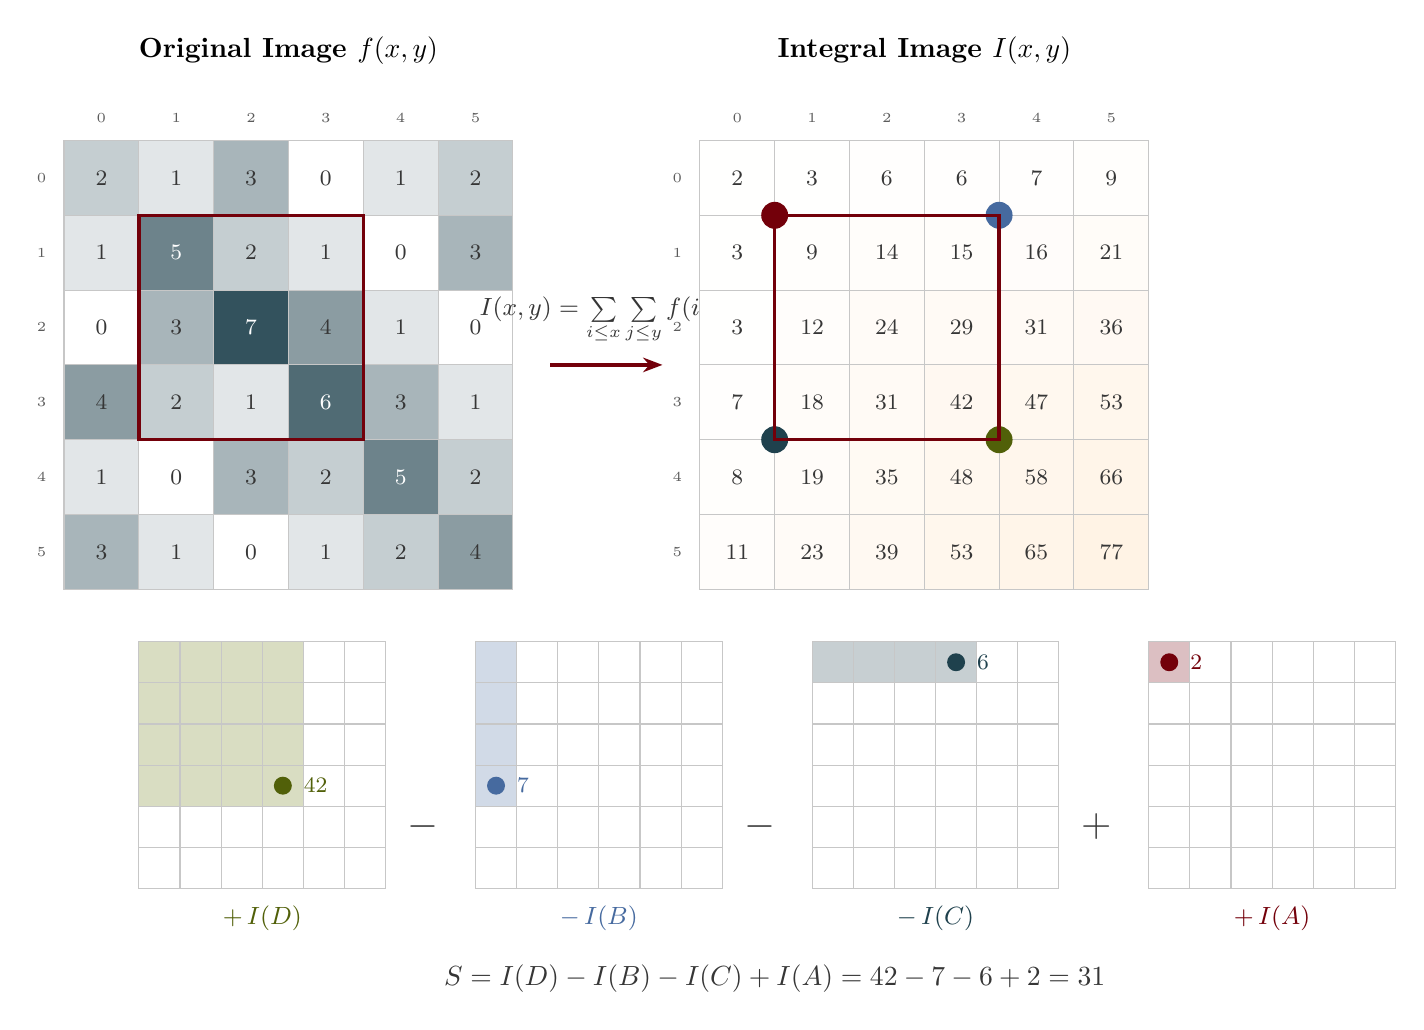
\begin{tikzpicture}[scale=0.95]

\node[font=\bfseries] at (3,7.2) {Original Image $f(x,y)$};
\def\ovals{{2,1,3,0,1,2,
             1,5,2,1,0,3,
             0,3,7,4,1,0,
             4,2,1,6,3,1,
             1,0,3,2,5,2,
             3,1,0,1,2,4}}

\foreach \r in {0,...,5}{
  \foreach \c in {0,...,5}{
    \pgfmathtruncatemacro{\idx}{\r*6+\c}
    \pgfmathtruncatemacro{\val}{\ovals[\idx]}
    \pgfmathsetmacro{\pct}{\val*13}
    \fill[congaree!\pct!white] (\c,5-\r) rectangle ++(1,1);
    \draw[gray30,thin] (\c,5-\r) rectangle ++(1,1);
    \pgfmathtruncatemacro{\bright}{(\val>4)?1:0}
    \ifnum\bright=1
      \node[font=\footnotesize,white] at (\c+0.5,5.5-\r) {\val};
    \else
      \node[font=\footnotesize,gray90] at (\c+0.5,5.5-\r) {\val};
    \fi
  }
}

\draw[garnet,very thick] (1,2) rectangle ++(3,3);

\foreach \c in {0,...,5}{
  \node[font=\tiny,gray70] at (\c+0.5,6.3) {\c};
}
\foreach \r in {0,...,5}{
  \node[font=\tiny,gray70] at (-0.3,5.5-\r) {\r};
}

\draw[-{Stealth[length=7pt]},very thick,garnet] (6.5,3) -- (8,3);
\node[font=\small,above,text=gray90] at (7.25,3.15) {$I(x,y) = \sum\limits_{i\le x}\sum\limits_{j\le y} f(i,j)$};

\node[font=\bfseries] at (11.5,7.2) {Integral Image $I(x,y)$};
\def\ivals{{2,3,6,6,7,9,
             3,9,14,15,16,21,
             3,12,24,29,31,36,
             7,18,31,42,47,53,
             8,19,35,48,58,66,
             11,23,39,53,65,77}}

\foreach \r in {0,...,5}{
  \foreach \c in {0,...,5}{
    \pgfmathtruncatemacro{\idx}{\r*6+\c}
    \pgfmathtruncatemacro{\val}{\ivals[\idx]}
    \pgfmathsetmacro{\pct}{min(\val*1.2,100)}
    \fill[sandstorm!\pct!white] (8.5+\c,5-\r) rectangle ++(1,1);
    \draw[gray30,thin] (8.5+\c,5-\r) rectangle ++(1,1);
    \node[font=\footnotesize,gray90] at (9+\c,5.5-\r) {\val};
  }
}

\foreach \c in {0,...,5}{
  \node[font=\tiny,gray70] at (9+\c,6.3) {\c};
}
\foreach \r in {0,...,5}{
  \node[font=\tiny,gray70] at (8.2,5.5-\r) {\r};
}

\fill[garnet] (9.5,5) circle (0.18);
\fill[atlantic] (12.5,5) circle (0.18);
\fill[congaree] (9.5,2) circle (0.18);
\fill[horseshoe!80!black] (12.5,2) circle (0.18);

\draw[garnet,very thick] (9.5,2) rectangle ++(3,3);

\begin{scope}[shift={(1,-4)}]
  \def\minisz{0.55}

  \begin{scope}[shift={(0,0)}]
    \foreach \r in {0,...,5}{
      \foreach \c in {0,...,5}{
        \pgfmathtruncatemacro{\inrect}{(\r<=3 && \c<=3)?1:0}
        \ifnum\inrect=1
          \fill[horseshoe!25] (\c*\minisz,5*\minisz-\r*\minisz) rectangle ++(\minisz,\minisz);
        \fi
        \draw[gray30,thin] (\c*\minisz,5*\minisz-\r*\minisz) rectangle ++(\minisz,\minisz);
      }
    }
    \node[font=\small,horseshoe!80!black] at (3*\minisz,-0.4) {$+\,I(D)$};
    \fill[horseshoe!80!black] (3*\minisz+\minisz/2, 5*\minisz-3*\minisz+\minisz/2) circle (0.12);
    \node[font=\footnotesize,horseshoe!80!black,right] at (3*\minisz+\minisz/2+0.15, 5*\minisz-3*\minisz+\minisz/2) {42};
  \end{scope}

  \begin{scope}[shift={(4.5,0)}]
    \foreach \r in {0,...,5}{
      \foreach \c in {0,...,5}{
        \pgfmathtruncatemacro{\inrect}{(\r<=3 && \c<=0)?1:0}
        \ifnum\inrect=1
          \fill[atlantic!25] (\c*\minisz,5*\minisz-\r*\minisz) rectangle ++(\minisz,\minisz);
        \fi
        \draw[gray30,thin] (\c*\minisz,5*\minisz-\r*\minisz) rectangle ++(\minisz,\minisz);
      }
    }
    \node[font=\small,atlantic] at (3*\minisz,-0.4) {$-\,I(B)$};
    \fill[atlantic] (0*\minisz+\minisz/2, 5*\minisz-3*\minisz+\minisz/2) circle (0.12);
    \node[font=\footnotesize,atlantic,right] at (0*\minisz+\minisz/2+0.15, 5*\minisz-3*\minisz+\minisz/2) {7};
  \end{scope}

  \begin{scope}[shift={(9,0)}]
    \foreach \r in {0,...,5}{
      \foreach \c in {0,...,5}{
        \pgfmathtruncatemacro{\inrect}{(\r<=0 && \c<=3)?1:0}
        \ifnum\inrect=1
          \fill[congaree!25] (\c*\minisz,5*\minisz-\r*\minisz) rectangle ++(\minisz,\minisz);
        \fi
        \draw[gray30,thin] (\c*\minisz,5*\minisz-\r*\minisz) rectangle ++(\minisz,\minisz);
      }
    }
    \node[font=\small,congaree] at (3*\minisz,-0.4) {$-\,I(C)$};
    \fill[congaree] (3*\minisz+\minisz/2, 5*\minisz-0*\minisz+\minisz/2) circle (0.12);
    \node[font=\footnotesize,congaree,right] at (3*\minisz+\minisz/2+0.15, 5*\minisz+\minisz/2) {6};
  \end{scope}

  \begin{scope}[shift={(13.5,0)}]
    \foreach \r in {0,...,5}{
      \foreach \c in {0,...,5}{
        \pgfmathtruncatemacro{\inrect}{(\r<=0 && \c<=0)?1:0}
        \ifnum\inrect=1
          \fill[garnet!25] (\c*\minisz,5*\minisz-\r*\minisz) rectangle ++(\minisz,\minisz);
        \fi
        \draw[gray30,thin] (\c*\minisz,5*\minisz-\r*\minisz) rectangle ++(\minisz,\minisz);
      }
    }
    \node[font=\small,garnet] at (3*\minisz,-0.4) {$+\,I(A)$};
    \fill[garnet] (\minisz/2, 5*\minisz+\minisz/2) circle (0.12);
    \node[font=\footnotesize,garnet,right] at (\minisz/2+0.15, 5*\minisz+\minisz/2) {2};
  \end{scope}

  \node[font=\Large,gray90] at (3.8,1.5*\minisz) {$-$};
  \node[font=\Large,gray90] at (8.3,1.5*\minisz) {$-$};
  \node[font=\Large,gray90] at (12.8,1.5*\minisz) {$+$};

  \node[font=\normalsize,gray90] at (8.5,-1.2)
    {$S = I(D) - I(B) - I(C) + I(A) = 42 - 7 - 6 + 2 = 31$};
\end{scope}

\end{tikzpicture}
\end{center}

\end{document}
